%% LyX 2.0.7.1 created this file.  For more info, see http://www.lyx.org/.
%% Do not edit unless you really know what you are doing.
\documentclass{article}
%\usepackage[T1]{fontenc}
%\usepackage[latin9]{inputenc}
%\usepackage{babel}
\usepackage{algpseudocode}
\usepackage{caption}
\usepackage[letterpaper, portrait, margin=1.1in]{geometry}

% ------- FOR PSEUDOCODE EXAMPLE ------------
% Documentation can be obtained here:
%  http://www.ctan.org/tex-archive/macros/latex/contrib/algorithm2e/
\usepackage[noend,ruled]{algorithm2e}
\usepackage{url}
\usepackage{graphicx}

\begin{document}

\title{CSC591/791 Advanced Algorithms Capstone Project:\\ 
       Streaming Dashboard for Journaling Data,\\
       and Review of Streaming Analysis Approaches}

\author{Paul Jones, pjones@ncsu.edu\\
        Dakota Medd, drmedd@ncsu.edu\\
        Kshitij Sharma, ksharma3@ncsu.edu\\
        Nitin Tak, ntak@ncsu.edu}

\date{May 5th, 2015}

\maketitle

\section{Instructions}

\begin{itemize}

\item \textit{Goal}: To dive into a particular area(s) presented in the course more in depth that appeals to advancing your professional/research career objectives.

\item \textit{Time and Teams}: The amount of time to complete the comprehensive exam or the capstone project is estimated to be approximately 20 hours (about 3 days of work); Teams are not required but teams of up to 5 students are allowed for the project. That means that the collective effort for a 5-member team is ~100 hours.

\item \textit{Topics}: MS/MR/BS (Kshitij and Nitin): Programming project that addresses a real application problem that requires end-to-end streaming or online algorithms (you may build by leveraging and extending the assignments you are doing in this class). At least one algorithm must be included in the project. PhD (Paul and Dakota): Either literature review of the algorithmic topic or the research development of the new algorithm of relevance to this course.

\end{itemize}

\section{Streaming Dashboard for Journaling Data}

This section describes the overall end-to-end implementation we have carried out for the Capstone project, and is designed to meet the documentation requirements for the Masters students on the team, as well as providing a general overview of what the team has done. Section 3 provides a thorough literature review of possible algorithms in our space of interest, which satisfies the requirements for the PhD students on the team.

\subsection{[Paul] Problem statement}

The main intention of this project is to \textbf{demonstrate real-time situational awareness capabilities for Journaling data}. The Journaling project is a research effort at the Laboratory for Analytic Sciences (LAS) that is aiming to systematically capture details of goals and tasks that knowledge workers are trying to accomplish. The idea is to be able to associate these with other instrumentation data, and to enable goal-driven recommendations, goal-driven search and other capabilities that should help people become more productive. The Journaling team are currently lacking any sort of real-time dashboard that displays the overall state of the data being generated, including event volumes, active users, popular URLs and documents, and so on. During March and April 2015, approximately 20 students from the Advanced Algorithms class (CSC591/791) at NCSU have been tagging documents and URLs with goals related to class assignments. This project will build a dashboard capability, and some initial streaming analysis algorithms, to help instructors maintain awareness of who is working on which assignments in the class, and also include some predictive capabilities.

\paragraph{}
We intend to do this by building upon many of the ideas taught in the class. By extending some of the early tutorials and Assignment 1 (covering a talk by Nathan Marz), we intend to build a demonstrator that uses the \textbf{Lambda architecture} to incorporate both streaming and batch approaches. Next, we plan to incorporate several interesting algorithms to extract insight from data. Along with a simple node.js/Socket.IO web dashboard (using knowledge gained in Tutorials 1 and 2), this will give us a complete end-to-end proof-of-concept demonstrator. 

\paragraph{}
At the same time, we will conduct a thorough \textbf{literature review of possible future approaches} to streaming analysis of Journaling data in order to meet the required challenges of the LAS. Finally, we will summarize some of these techniques and recommend algorithmic approaches that could be explored in the future.

\subsection{[All] Learning objectives (i.e., why you are doing this, what you expect to learn, and how this topic fits in with the overall course objectives)}

We had the following learning objectives in mind when deciding to do this project:

\begin{itemize}

	\item Demonstrate some algorithms relevant to this course on real-world data that is generated by the class (the Journaling data in itself can be considered a diarization of the work carried out for the class). Through this exercise, we aim to \textbf{understand the limitations of these algorithms when applied to real-world data} - we expect them to break down in certain circumstances, which will provide valuable learning opportunities.
	\item Focus on streaming analysis techniques and approaches that can deliver situational awareness of the class through the Journaling data in close to real-time, whilst at the same time integrating batch approaches (in a style similar to the Lambda architecture) as appropriate. As a result, we aim to \textbf{deepen our understanding of the constraints and opportunities presented by streaming algorithms}, including some predictive approaches.
	\item Provide the foundations for a \textbf{dashboard} that will hopefully be useful to course participants and instructors, and that will be further developed for the Journaling project after this Capstone project is complete. Through this, we hope to \textbf{learn what it takes to deliver a complex and useful capability in a short period of time}.
	
\end{itemize}

\subsection{[All] Description of algorithm(s) used}

During this project, we have used the following algorithms (see Section 3 for justification of why we chose these, and for a survey of related algorithms):

\begin{itemize}

	\item \textbf{Holt-Winters} (HW) for forecasting level-of-activity of users: the HW algorithm assumes a model for time series that includes terms for weighted moving average, trend, and seasonality. This type of model is well-suited to Journaling data since: (1) we expect user behavior to change over time (hence the need for a weighted moving average), (2) we expect a trend in the data, since individual users may submit more data later in the experiment, and (3) we expect seasonality in the data on multiple timescales (certainly daily and weekly). 

    \item \textbf{Association-Rules} as a first step to being able to predict or recommend URLs: Association Rules algorithms attempt are two-step algorithms that attempt to find frequent items that have a minimum frequency, and then from these sets generate a set of rules of the form $S \rightarrow I$, where $I$ is some element in a frequent set $F$, and $S=F-I$. After these rules are generated, the algorithm then filters out the rules that are not interesting, usually by testing the frequency against some noise baseline. For the traditional Apriori association rule mining algorithm, this baseline is the frequency of $S$.
    
    \item \textbf{Top-k Heavy Hitters} as a streaming approximation of association rules: The top-k heavy hitters problem is concerned with finding the most frequent items that occurred within a stream. To accomplish this, the algorithm keeps a priority queue (a normal array whose order is maintained by insertion sort) of the most frequent elements, and when a new element is encountered, the count of the element is checked. If the new element's count is greater than the smallest element of the queue, and the new element is not already in the queue, the smallest element is dequeued and the new element is enqueued. The counts of each element are maintained with a count-min sketch. A count-min sketch is an $h$ by $d$ array that approximates the count of each element. When a new element arrives, the element is passed through $h$ hash functions (one for each array) to generate an index into each array. Each $h$ value is then incremented by one. To get the count of an element, the element is again hashed by the $h$ hash functions to index the array and retrieve the $h$ values. From here, the minimum of these values is returned as an approximation of the count of the element.

\end{itemize}

\subsection{[All] Description of implementation details}

\paragraph{}
Our goal with the streaming dashboard is to provide knowledge workers with aggregate data in real-time that describes user actions to improve both situational awareness and to help promote the establishment of a set of best-practices. The methods chosen to generate these aggregate results must be accurate in order to ensure the best course of action is taken. The algorithm we chose for this is the NB-frequent itemset algorithm (see section 3 for reference), due to it being able to detect and report rare events. However, this method, while applying filtering rules, can quickly grow in complexity as the number of records increase. This will cause our aggregations to quickly become outdated. To solve this issue, we chose to use the lambda architecture paradigm discussed in the talk by Marz \cite{marztalk}.

\paragraph{}
\textbf{Lambda architectures} are a system design paradigm that calls for a two-tier data processing pipeline for handling streaming data. The first tier of processing (the near real-time component) operates in a streaming fashion by receiving the data stream one element at a time and producing temporary results with some allowable error. For this portion, we chose to implement the heavy hitters algorithm, discussed in section \textbf{2.3}. The second tier of processing (the batch component) also receives the data stream one element at a time, in parallel with the streaming portion. However, instead of operating in a streaming fashion, the elements are stored in permanent storage and the data is operated on in batchs. Usually, this batch algorithm is allowed to be slow but needs to be accurate. Items that are added to permanent storage during the batch algorithm's execution are not considered. For our system, we chose the NB-frequent itemset algorithm discussed in section \textbf{2.3} as our batch component.

\paragraph{}
When a user polls a lambda architecture pipeline for an answer to a query, the architecture first determines if the query can be answered just through the old answers of the previous batch run. If they can, the pipeline will return these answers. However, if the query requires new data that did not exist in the old batch algorithm's corpus, the pipeline returns the temporary value calculated in the streaming component. For our system, we felt this type of logic should not be used. Instead, the knowledge worker should have access to both the newer (possibly error-prone streaming) answer, and the older answer (which is possibly slightly out-of-date). This way, the analyst can use their own discretion in choosing which answer is more meaningful.

\paragraph{}
Our implementation of this lambda architecture is divided into multiple modules integrated together to collectively demonstrate real-time situational awareness capabilities for Journaling data. These modules can be categorized as follows:

\begin{itemize}

\item \textbf{R-Scripts}: The core modules responsible for performing all the analytical activity to gain insights on the real-time streaming data including streaming predictive analysis to enable recommendation and situational awareness. These are standalone R Scripts which are invoked by a node.js server (explained below) to execute and save their output in the form of `.png' images. These modules are called from the server on user invocation. Running as a back-end process for the application, these modules generate Activity Plots, Support-Confidence plots, and graphical plots from the Apriori association rules, depending on user selections available on the dashboard. The dashboard displays the `.png' generated by these scripts to the end users.

\item \textbf{node.js server}: This is the binding element for the entire project which integrates all the modules. The node.js server is responsible for running the R-scripts based on user selection from the dashboard. It also facilitates all communication between the server and the dashboard using Socket.IO calls. The modules that run external to node.js become child processes and are spawned from the node.js server itself. It is the outcome of these processes that is displayed on the dashboard using socket communication.

\item \textbf{Dashboard}: We have created a dashboard that provides several functionalities:
\begin{itemize}
\item ``Tell me more": This button gives the user an option to view and understand about what the dashboard is about and how to interpret it.
\item ``Filter by User": This enables the user of the application to select a particular trial participant and run the time series and Apriori analytics for that student. When the student is selected, all the assignments are considered for that particular individual. The results are then populated on the dashboard.
\item ``Filter by Assignment": Similar to ``Filter by User", this enables the user of the application to select a particular class assignment and run the time series and Apriori analytics based on all the data for that assignment. When the assignment is selected, all the students are considered for that particular assignment. The results are then populated on the dashboard.

\end{itemize}

\item Additionally, we implemented the \textbf{Top-k Heavy-Hitters algorithm} from scratch on the node.js server using CountMin Sketch and Priority Queues. Journaling data is obtained from an NCSU server by calling a REST API. The response is rendered in JSON format and parsed into transactions, which form the input to the frequent itemset algorithm, which we also implemented from scratch. A transaction in our context is a list of URLs that a user accesses within a short time period. Pseudo code for the algorithm is below:

\end{itemize}

\paragraph{}
\textbf{GENERATING N-FREQUENT ITEMSETS}

\begin{enumerate}

\item Fetch history of user activity from LAS server
\item Process data and create a list of transactions Ti
\item Count the support of URL’s from each transaction and store in a TopK data structure 
\item For i= 2 .... N // Generate N-frequent itemsets.
\item \hspace{1cm} $C_i$ = Generate candidate i-itemsets 
\item \hspace{1cm} For each transaction $T_i$
\item \hspace{1cm} \hspace{1cm} Prune candidates which are not contained in any Transaction. 
\item Return $C_n$ // n-set frequent item sets


\paragraph{}
\textbf{GENERATING CANDIDATE ITEMSETS}

	\item For each item $i_k$ in $C_k$
	\item \hspace{1cm} Generate all k-1 item subsets $s_{k-1}$ for each $i_k$
	\item \hspace{1cm} \hspace{1cm} Remove $i_k$ from $C_k$ if $s_{k-1}$ $\notin$ $i_k$ 
	\item Return $C_k$ // $C_k$ = pruned k-frequent item sets.
\end{enumerate}

\paragraph{}
\textbf{Analysis of the algorithm}: Processing data at step 2 of the algorithm has a complexity of $O(hn)$ where $h$ is the number of hash functions for the CM sketch, and $n$ is the number of URLs. We iterate through each URL once and create transactions. In step 3, we iterate through each transaction and count the support of each transaction and store it in a count-min sketch. We implemented a top-k priory queue using an array implementation and insertion sort. Insertion into the queue could be $O(nk^2)$ worst case. 

\paragraph{}
We could considerably improve the performance to $O(nlog(k))$ by implementing the Priority Queue using Heap and, using Fibonnaci heaps, it could be amortized (averaged to) $O(1)$. At step 4 we implement the N-frequent item-set. Its implementation is defined in lines 9 to 12. Generating $k-1$-itemset subsets of $i_k$ is exponential in terms of $k$. In worst case, it could be $O(k!)$. But, in practice, specifically in our case $k$ is small (typically somewhere between 3 and 4) so its effect on the performance is relatively small. At line 11, we prune the infrequent item-sets using the anti-monocity principle of the transaction. At line 7, we further eliminate infrequent item-sets by comparing them against each transaction. In lines 4 to 7, the complexity of our algorithm is $O(n^4)$, assuming that generating $k-1$-item subsets does not dominate.

\pagebreak

\subsection{[Paul] Description of experimental design}

In order to test these algorithms as part of the overall Journaling prototype, we integrated them into the system as shown in Figure 1.

\begin{figure}[ht!]
\centering
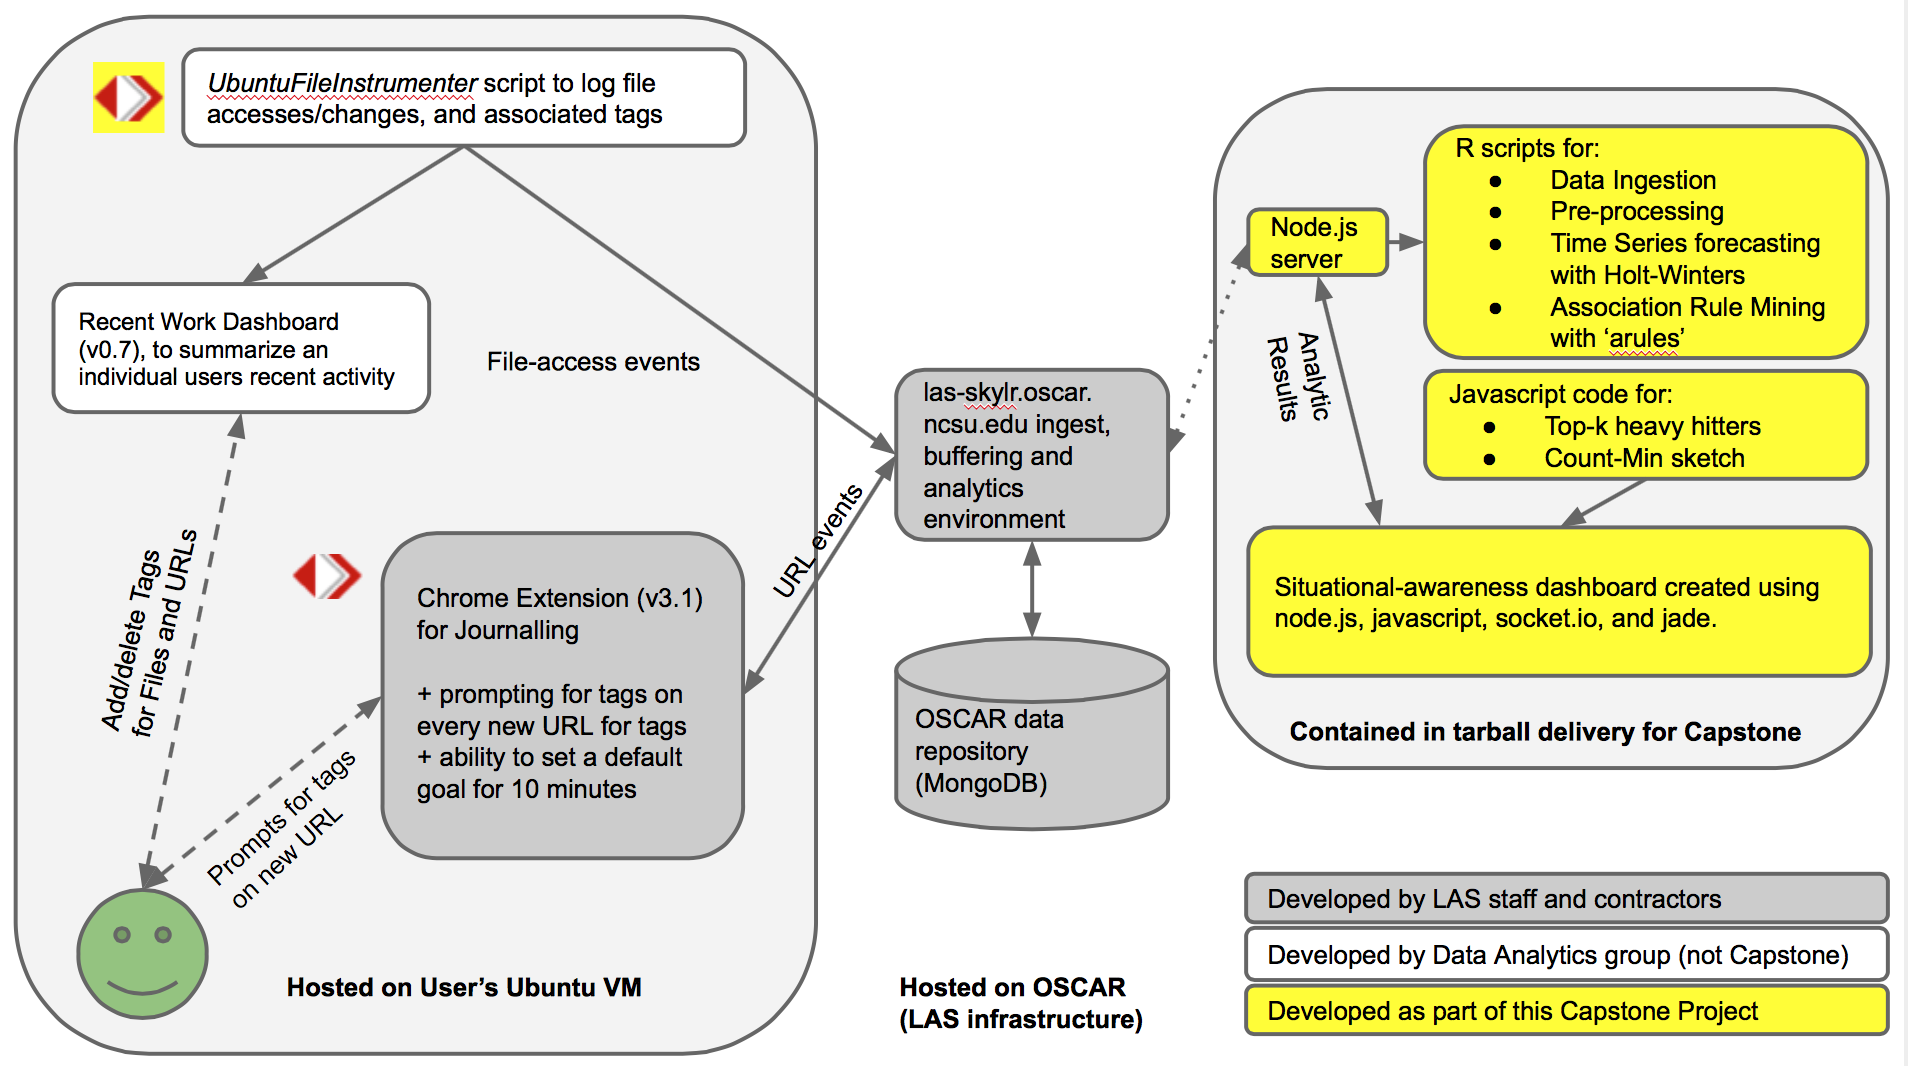
\includegraphics[width=170mm]{images/capstone-diagram.png}
\label{diagram}
\caption{System Diagram for CSC591/791 Class Journaling trial on Ubuntu with analytics (in both R and Javascript) for Situational Awareness Dashboard created for Capstone Project (as at May 5th, 2015)
}
\end{figure}


\paragraph{}
The data we are analyzing is derived from Instrumentation running in each participant's Ubuntu Virtual Machine (VM) - this consists of a Chrome-based extension that prompts for user goals each time a new URL is accessed, and also an \textit{UbuntuFileInstrumenter} script that detects file accesses and edits. In each case, and event record is created (in JSON format) and sent to LAS infrastructure (Oscar) where it is processed and stored in a MongoDB database. There is also a `Recent-Work Dashboard' component developed by the Data Analytics Group (but not part of this Capstone project), which was made available to trial participants.

\paragraph{}
For this project, we query the Oscar infrastructure either for a batch pull from the MongoDB database, or for a live feed of data direct from the Kafka ingest buffering. Everything developed for the Capstone project is self-contained in that it will run on any Ubuntu (or other Linux) platform, and is only dependent on the REST API available provided by \texttt{las-skylr.oscar.ncsu.edu}. The source code contains a static AuthToken that is used to authenticate with the server - hence no user configuration is required; once software dependencies are installed, our analytics should work `out of the box'.

\paragraph{}
This platform allows us to achieve the learning objectives listed in section 2.2, as well as delivering a useful component to the LAS Journaling project.

\subsection{[Dakota] Analysis of results}

\paragraph{}
After processing the activity logs of the 20 students, we found that most results of the batch Apriori algorithm fell into three classes, illustrated in Figures 2(a), 3(a) and 4(a) with associated distribution of activities shown in Figures 2(b), 3(b) and 4(b). 

\begin{figure}[ht!]
\centering
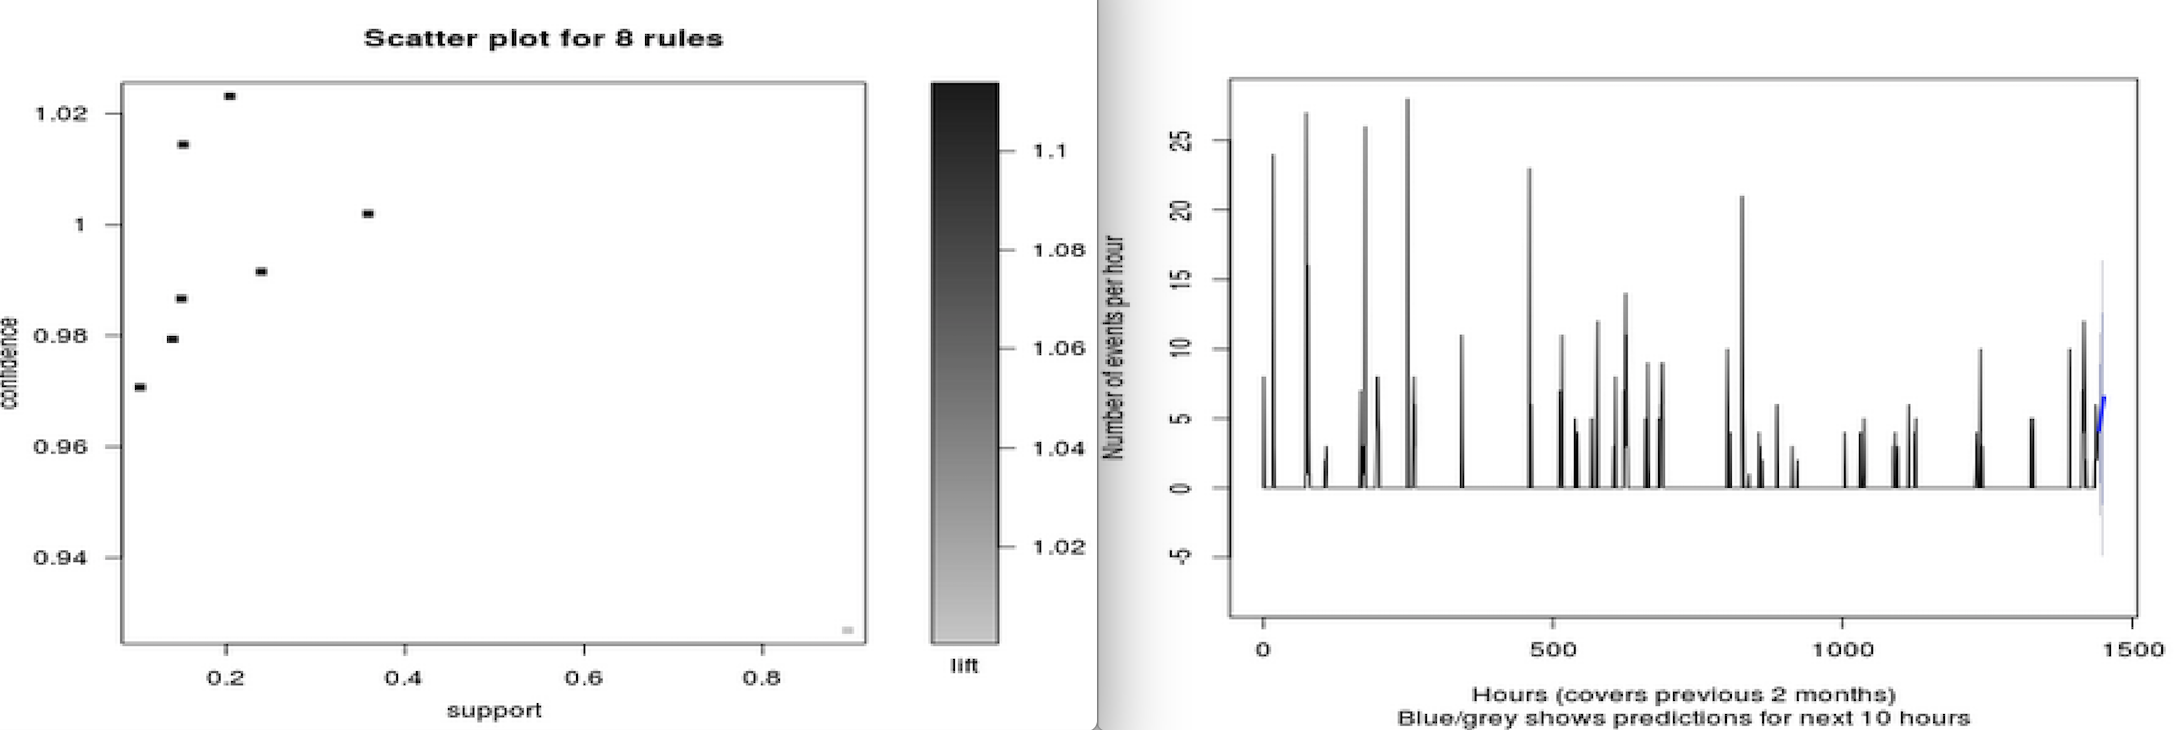
\includegraphics[width=170mm]{images/fig-2.png}
\label{diagram}
\caption{(a) Apriori scatter plot, and (b) associated activity timeline for user `pjones'}
\end{figure}

\paragraph{}
Figure 2 shows the results for a user with regular periodic activity spread throughout the time windows. The results from our batch Apriori algorithm are straight-forward, producing clean results. This is due to the uniform nature of the data points generated by this student. However, the distribution of activities for some other students are not as uniform. 

\begin{figure}[ht!]
\centering
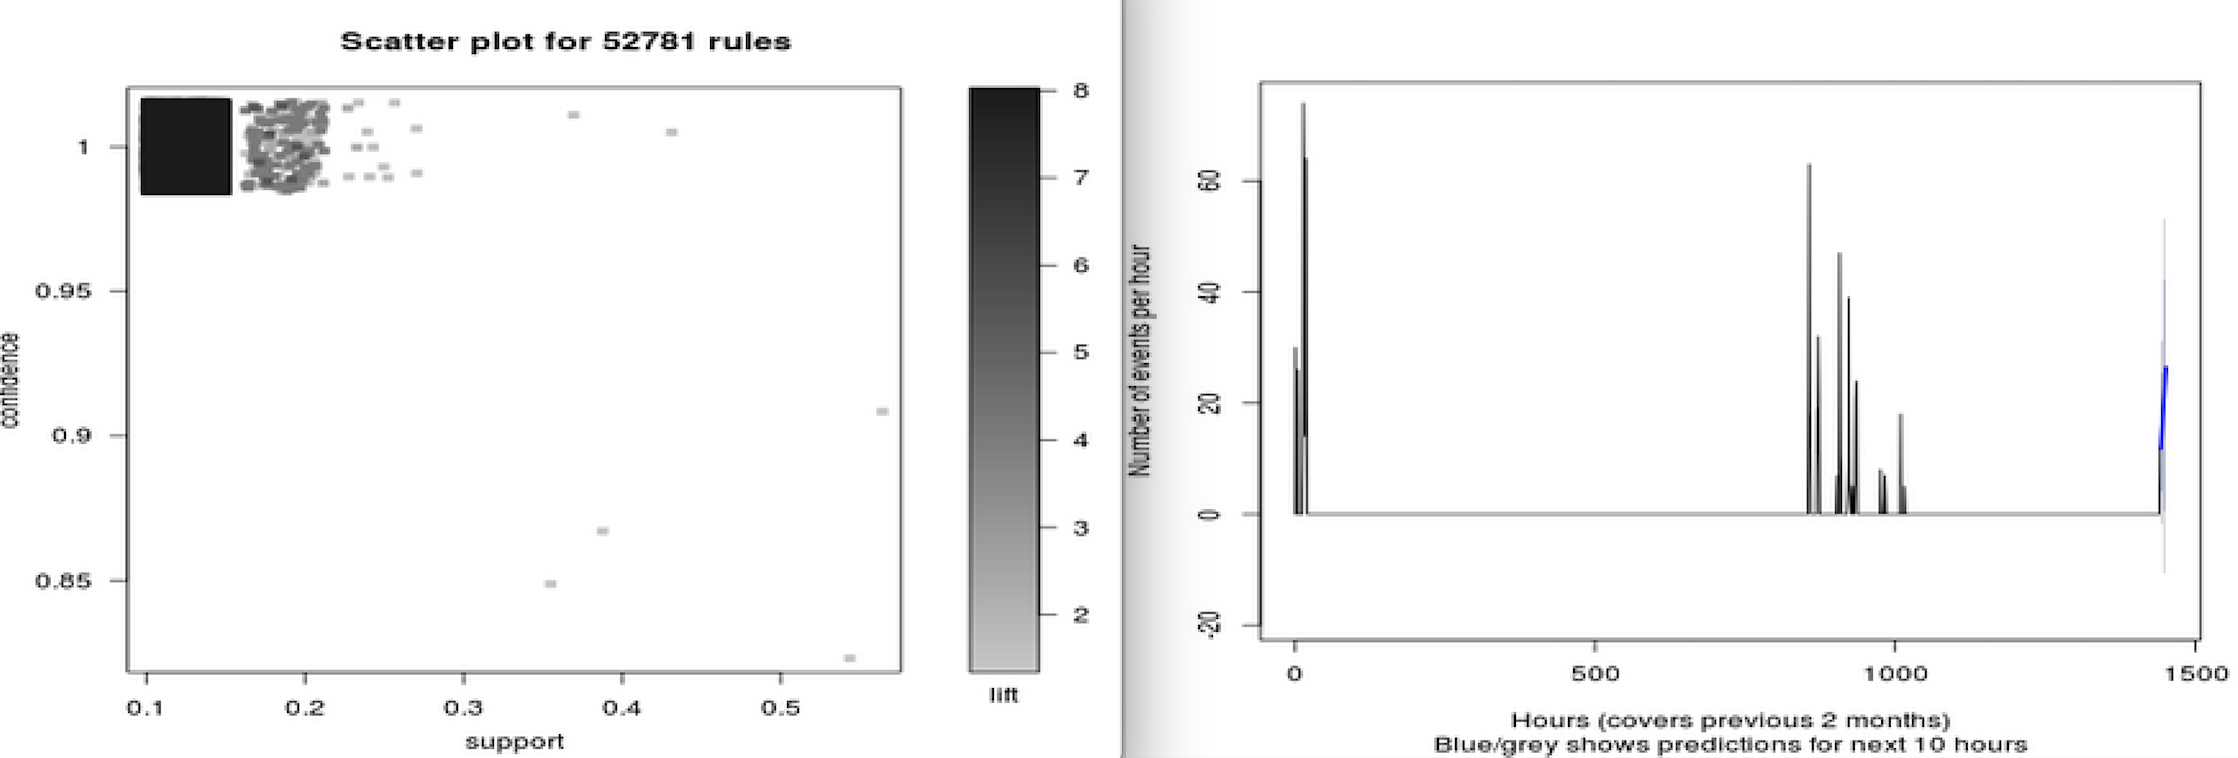
\includegraphics[width=170mm]{images/fig-3.png}
\label{diagram}
\caption{(a) Apriori scatter plot, and (b) associated activity timeline for user `drmedd'}
\end{figure}

\begin{figure}[ht!]
\centering
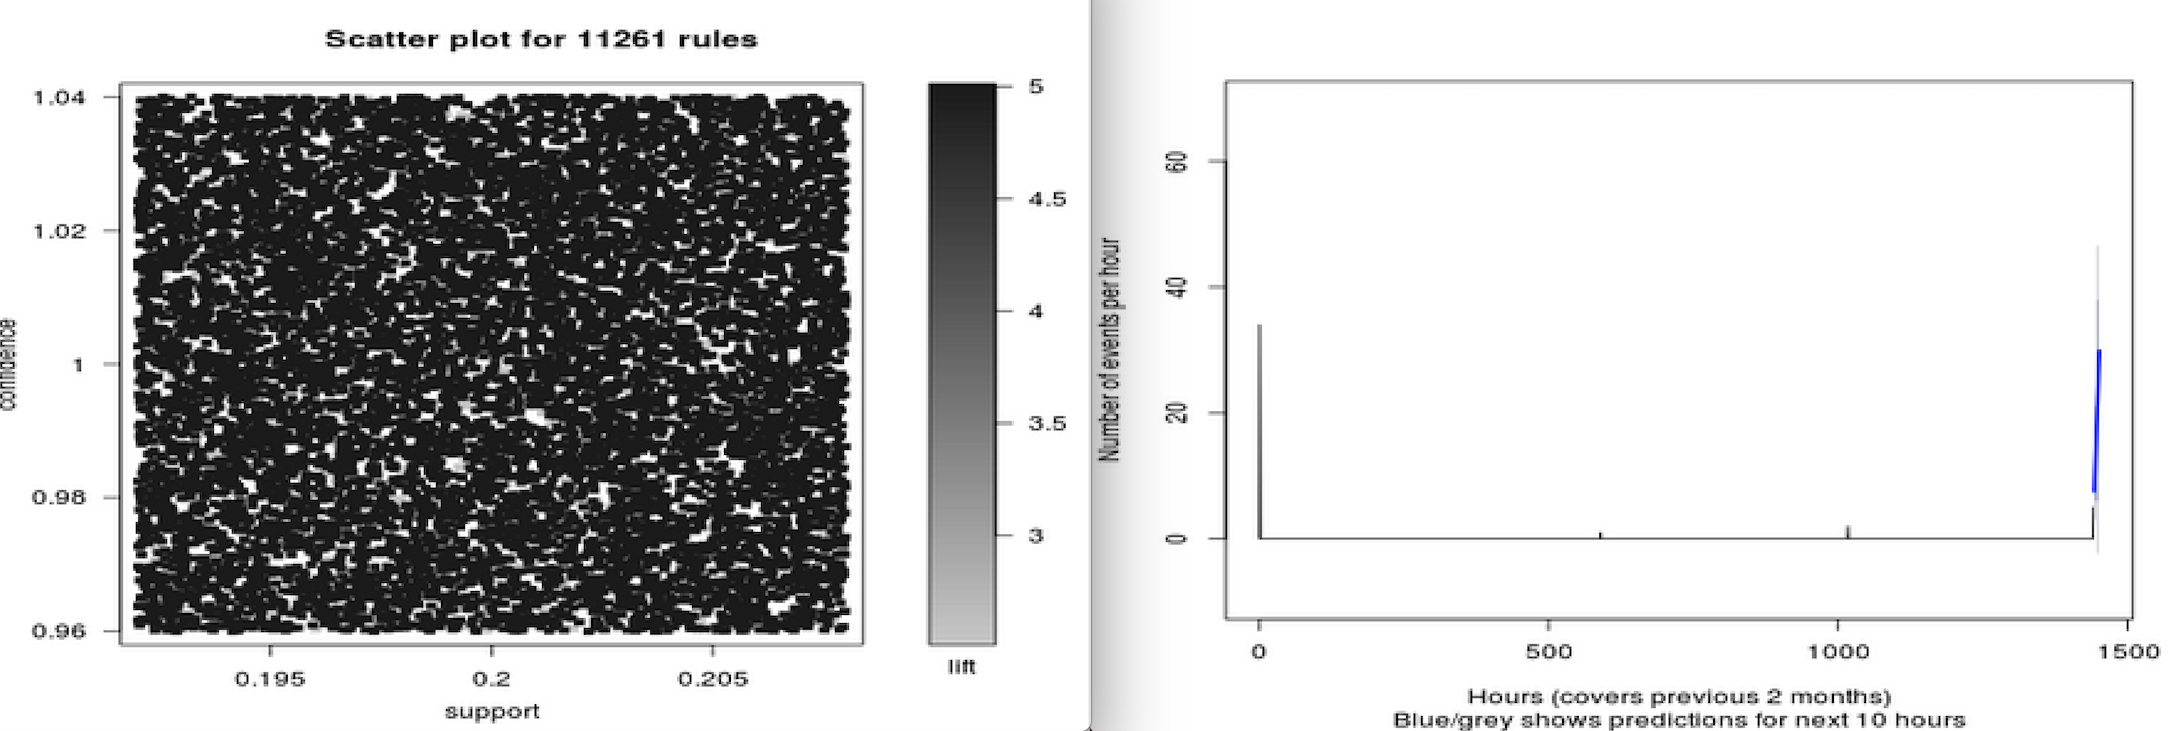
\includegraphics[width=170mm]{images/fig-4.png}
\label{diagram}
\caption{(a) Apriori scatter plot, and (b) associated activity timeline for user `shsu3'}
\end{figure}

\paragraph{}
In the case of Figure 3, the user's actions are sporadic, characterized by bursts of intense activities separated by long dead spaces. For this case, which we have denoted as \textbf{semi-degenerate}, the user's activity is structured and focused on completing a single task. Therefore, most transactions will be significant, having many duplicate transactions. This will lead to high Support (frequency of observed link between items) and also high Confidence (the ratio of associated item with original item). 

\paragraph{}
In the case of Figure 4, the user's activity appears to be bimodal but, in general, the levels of activity are unstructured and infrequent. This case is \textbf{degenerate}, and produces multiple rules of varying confidence, because there aren't enough meaningful transactions to find any meaningful results. This leads to low support and confidence for all rules, which means that many spurious rules get considered (i.e. it cannot distinguish a signal from the noise).

\subsection{[All] Discussion of lessons learned}

As a result of implementing all of the techniques against real-world data, and in a streaming setting, we have learned a number of interesting lessons.

\paragraph{}
Firstly, from prediction of activity levels in time series data, we have learned that there are many different approaches to this - the one we attempted (Holt-Winters) seems like a good fit and, at least by eye, appeared to generate sensible predictions in most cases. It tended to break down in situations where data was bursty and aperiodic. However, a detailed empirical performance evaluation has not been carried out as part of this project.

\paragraph{}
The bursty and aperiodic nature of our data also seems to have adversely effected the association rules we mined using Apriori. This may indicate that, in all cases, we might want to attempt to identify such characteristics in data, and apply different methods accordingly. 

\paragraph{}
From our implementation of association rules in a batch mode, we observed large computation times, even with our relatively low-rate data. From this, we identified that a need does indeed exist for separate streaming and batch approaches (i.e. a Lambda architecture). This allows an approximation to the association rules to be provided quickly even when the batch algorithm is still running. For this, we found that an approximation based on identifying the current top-k heavy hitters was likely to be good enough to provide an initial recommendation to a knowledge worker.

\paragraph{}
Finally, we experienced that developing streaming dashboards is a time-consuming process - however, the technologies we learned about in Project 1 helped us with this considerably. We implemented both polling (for static files), and streaming connections (based on Socket.IO). This made the value of web sockets technology very clear to us. As further work, it would be good to transition the file-polling parts of the dashboard to Socket.IO in due course.

\section{Review of Streaming Analysis Approaches for Journaling Data}

\textit{[Joint effort between Paul Jones and Dakota Medd; all text is our own, except where quoted and explicitly referenced; all sections labelled according to main author; all sources referenced.]}

\paragraph{}
The current trial of the LAS Journaling prototype (for DO4) attempts to systematically associate CSC791 class-related goals with documents and URLs. All events consist of a goal that relates to a specific assignment and activity (e.g. CSC791AdvAlg\_Project\_P5\_Writing). Each has an associated document filename or URL.

\paragraph{}
There are several immediate requirements for streaming predictive analytics on the current Journaling data, all of which are essential to enabling future recommendation and situational awareness capabilities. The analytics considered here are candidate approaches for the following:

\begin{itemize}
	
	\item \textbf{Level-of-Activity Prediction} - we would like to know when each student will probably next be active (e.g. so we can prepare recommendations), and when there will likely next be activity for a given assignment.

	\item \textbf{Next-Activity Prediction} - we would like to know which document or URL a given individual is likely to want to access next; with this information, the system could pro-actively download or access the URL in advance of the user requesting it.

	\item \textbf{Goal Recognition} - we would like to be able to label any new document or URL with a predicted goal to avoid having to prompt the user to do this manually. In addition, the system can only make sensible recommendations when it has some awareness of the user's intended end-goal.

\end{itemize}

Each of these capabilities is now considered in turn, along with some candidate approaches. Note that this survey is by no means intended to be comprehensive!

\subsection{Approaches for Level-of-Activity Prediction} 

\subsubsection{[Paul] Time Series Analysis}

Given a continuous stream of real-valued data points on one variable (univariate) derived from the Journaling data (e.g. number of events submitted in a given time interval), there are a number of standard statistical approaches that can be applied to forecast the likely value of a data point at some time in the future. These methods typically date back to the 1980s or earlier, so it is difficult to find the original sources. Perhaps the simplest technique is the \textbf{Moving Average} (MA) model, which is just a linear regression over the data stream so far. Another very common model is the \textbf{AutoRegressive} (AR) model, which assumes that the output value depends linearly on some combination of its own previous values. These can be combined with an \textbf{Integrated} (difference) term, which removes any trend and produces a stationary (mean-reverting) time series. We can combine all of these model components into a very general class of time series forecasting models called ARIMA \cite{melard1984algorithm}.

\paragraph{}
Instead of weighting past observations equally (as in the case of simple MA), we can assign exponentially decreasing weights over time to produce an \textbf{Exponential Smoothing} model. These models do not typically do well when there is an overall trend or seasonality in the data, so additional exponential smoothing terms are often included to take these into account. Such a model that includes terms for weighted moving average, trend, and seasonality are known as \textbf{Holt-Winters} models. This type is model is particularly appropriate for long-term forecasting on the Journaling data since: (1) we would expect user behavior to change over time (hence the need for a weighted moving average), (2) we would expect an overall trend in the data, since individual users may submit more data when they become more confident, or when more users are added to the experiment, and (3) we would expect seasonality in the data on multiple timescales (certainly daily and weekly). For these reasons, Holt-Winters is a good candidate for forecasting likely levels of activity on Journaling data, at some arbitrary time in the future.

\paragraph{}
More recently, researchers have demonstrated the use of \textbf{Support Vector Machines} (SVM)s for time series modeling. The advantage of these is that, through the use of a suitable kernel, they can find interesting non-linear patterns in the data. However, SVMs have a tendency to overfit to complex time series and finding an optimal model can be a time consuming process. For this reason, people are moving towards other machine learning approaches, which can learn arbitrary patterns of data, and at different resolutions. 

\paragraph{}
The recent surge of interest in \textbf{Deep Learning} techniques, which typically use unsupervised feature learning at the lower levels of the hierarchy, are gaining increasing attention in the field of time series modeling \cite{langkvist2014review}. These can often learn better features than any that could be hand-crafted. Of these models, one of the most common building-blocks is the Restricted Boltzmann Machine (RBM), first described in \cite{hinton2006reducing}. This is a simple neural-network model that uses multiple layers of visible and hidden units, and an energy function to model the probability distribution over the inputs. These approaches are still in their infancy for analysis of time series data, and are more commonly used on sequence or multimedia data (e.g. for object recognition). As such they are considered further in this review as a possible approach to `goal recognition' on the Journaling data.

\subsubsection{[Dakota] Poisson Process}

The field of queueing theory has been dealing with issues of workflow profiling and approximation for decades. A common technique to approximate the behavior of real systems is the creation of a \textbf{stochastic process}, a collection of random variables whose values evolve over time \cite{psmrotar}. One of the most simple stochastic processes is \textbf{fixed-interval homogeneous counting processes}. Formally, a fixed-interval counting process $N_t$ is defined as a probabilistic equation that counts the number of times a given element has occurred and satisfies these constraints \cite[p.~308]{pspflor}:

\begin{enumerate}
	\item $N_0=0$, or the count starts at zero
	\item $N_t$ is monotonically increasing (i.e. the total number of occurrences doesn't decrease)
	\item $N_t$ is homogeneous, meaning the rate of occurrences for a given window is the same for all windows
	\item The increase of elements that occur within a given fixed window is independent of any other fixed window
	\item For a given fixed window of time, we assume only one occurence of an element occurs (Rare event law)
\end{enumerate}

Now, with these defintions, we can prove that for a given time window, the count of elements follows a Poisson distribution with a latent flow factor of $\lambda$, which represents the mean or rate of occurrence. This is because a Possion distribution has a built-in memoryless assumption \cite{psmrotar}. For this reason, stochastic processes that satisfy these constraints are usually called \textbf{Homogeneous Poisson Processes}. However, this distribution only gives us the probability of the value for a given time unit. To get the probability of the count equaling a given value over a specific range of windows, we can just simply extend the defintion to say that the total count over a given range of length $\delta$ follows a Poisson distribution with a latent flow factor of $\lambda \delta$, which would mean we expect the the count to just be the expected number of windows that equaled 1. While this process is very simple, it has been shown to be applicable in a variety of real world scenarios, such as finance, customer arrival, etc \cite{hahsler2006model}.

\paragraph{}
While Poisson processes are simple, an issue that makes them potentially unreliable for the Journaling domain is the independence in the count between any two fixed time windows. While the property of independence might be realistic for analysis across different assignments, it is not realistic for the high-grain action-by-action model we have adopted for analyzing Journaling data.  However, these simplifications do allow for Poisson distributions to be used as a baseline of evaluation for other metrics, such as `interest'. This is the approach used in Hahsler \cite{hahsler2006model}, which we will discuss in section \textbf{3.2.2}. To create a more robust baseline, Hahsler and others usually extend the homogeneous Poisson process to a dynamic heterogeneous model.

\paragraph{}
A \textbf{Heterogeneous Possion Processes} is a Possion processes where the latent flow variable is a function of time, or $\lambda(t)$. While this extension is simple to account for at any given window $t$, (it is just $\lambda(t)$), for a window of values this becomes more complex, usually requiring we solve some integral over the window change. We can introduce a similar change to allow for a \textbf{marked Poisson Process}, which allows you to associate some kind of marking for the flow of the Poisson process. This is usually introduced by just multiplying the latent factor by some kind of probability. Now, suppose the probability of a particular event occurring is also pulled from some distribution. This is called a stochastic mixture model, and serves as the basis for incredibly sophisticated methods, such as the computation of the baseline for NB-frequent item sets (discussed in section \textbf{3.2.2}) or LDA (discussed in section \textbf{3.3.3}).


\subsection{Approaches for Next-Activity Prediction} 

\subsubsection{[Dakota] Sequence Prediction}

\paragraph{}
Sequence prediction algorithms are algorithms interested in finding the next activity in a sequence of activities given a previous history of values called the \textbf{context}. The most simple way to approach this problem is through the use of a stochastic processes, like the Poisson process discussed in section \textbf{3.1.2}. However, Poisson processes are too simplistic for this task. Instead, we can use \textbf{Hidden Markov Models} (HMM). HMMs are a common machine learning approach to predicting the next character in a sequence of characters, given some static history length $k$. An HMM that uses $k$ previous elements to determine the next element in a sequence is called a $k$-order Markov Model. Fundamentally, these models assume the sequences are a result of a set of previous actions determined by the order, and the state of some hidden latent variable controlling the sequence. While commonplace and useful, HMMs have a large set of shortcomings. HMMs can be viewed algebraically as adjusting values in a set $k+1$ dimensional matrices, making both space needed to store the HMM and the complexity of training the algorithm grow polynomially on the size of context. The number of latent variables must be known in advance, which might be impossible for complex data, requiring approximation of this value through multiple training sessions, thereby further increasing the computational time. In addition, the same length of context is used for every possible value of an element in a sequence, which when studying and predicting dynamic Journalling behavior, will lead to some error. Finally, once a HMM is trained on a dataset, it cannot be retrained, introducing the notion of concept drift. Therefore, while HMMs are a common approach, other methods of estimation need to be used in the domain of Journalling.

\paragraph{}
One alternative to just applying HMMs on the sequence of elements is the notion of building a \textbf{context tree} \cite{dekel2009individual}. A context tree is a tree that encodes the sets of contexts, or suffixes, encountered previously by the algorithm. Usually, the nodes in the context tree represent some element in the alphabet of encountered elements, with a child for every element that occurred after the parent. Some algorithms reverse this ordering, however functionally they are constructed in the same way. To predict the next value, some prediction function is applied on the tree, which usually has embedded within it some values to aid prediction. \textbf{FxL} and \textbf{Adaptive FxL} \cite{hartmann2007prediction} are algorithms that build a context tree of all the sets previously encountered, and using the frequencies of the sets encoded within the tree along with standard bayesian rules, predict the probability of a symbol $x$ occurring next in the sequence. While these algorithms do overcome some limitations of HMMs (mainly by replacing a fixed context with a context whose length can be at most $d$), these methods still require a large memory footprint, and restrict the size of the context to some constant value. The \textbf{Shallow Perceptron model} of sequence prediction by Dekel et. al \cite{dekel2009individual}, attempts to fix this by projecting the context tree generated by reading substrings of the sequences into the real number space. They then prove this projection turns the problem of sequence prediction to that of linear separability, which they solve using perceptrons, or simple neural networks. Neural Networks relate heavily to the topics of Deep Learning, which will be discussed in section \textbf{3.3.3}. To control the growth of the tree (or in this case the perceptron built to operate on the projected tree), they add a controlling factor that limits growth of the tree by some logarithmic factor. 
 
\subsubsection{[Dakota/Kshitij] Association Rule Mining}

\paragraph{}

Association Rule Mining (ARM) is a traditional data mining task that emerged from early market basket analysis to answer questions about directional correlation in the purchasing history of users. For example, milk, eggs, diapers and beer are common items bought a grocery store. Through techniques that just measure the frequency of items, we will most likely find these items appearing together. However, when we measure directional correlation, or the likelihood of finding one element given the presence of another element, we find that customers that usually buy diapers also buy beer. We can find these relations through Association Rule Mining, which attempts to find relations of the data in the form of: what is the likelihood of finding element $I$, given element $J$? While not as sophisticated as most sequence prediction techniques, ARM algorithms are usually easy to understand and do not operate as a blackbox. Therefore, their results are more easily understood by non-technical users, allowing for a higher rate of adoption.

\paragraph{}
Historically, this problem is solved using a modified version of the \textbf{Apriori algorithm} \cite{agrawal1994fast}, an algorithm that intelligently enumerates all subsets of items that occur in the full history of transactions. The process of enumeration begins by scanning through the database and extracting all the singletons (sets of size one) that meet a certain frequency threshold $\lambda$. After this base case is formed, the algorithm works by taking sets of length $l-1$ and forming possible candidate sets of length $l$, which are then checked against the database. Those elements that meet $\lambda$ are saved. After this algorithm is run, association rules of the form $S \rightarrow I$, where $S$ is a set of elements and $I$ is a singleton set of elements, are formed with the counts found in the Apriori step.

\paragraph{}
The primary metric for quality in the Apriori algorithm is \textbf{support}. For a rule to be good in the Apriori algorithm, the support for the rule must be greater than some threshold. Support is simply the frequency of all the items occurring together in the database (or freq($S \cup I$). Once a rule meets this requirement, the confidence of the rule is then checked to ensure it meets a minimum threshold. The confidence of a rule is calculated by taking the support and dividing it by the frequency of $S$. While this method is useful because it is easy to compute, as outlined by Hahsler \cite{hahsler2006model}, there are some shortcomings. These include support biasing short rules, filtering out interesting but infrequent rules and finding misleading associations between very common elements. Therefore, Hahsler proposes a shift to a model that uses a metric that utilizes more robust statistical methods to characterize more of the underlying statistical properties of the dataset. In his case, he chooses to model the occurrences of elements within a given record by a Poisson process. Then, by using the counts and probabilities of a pair of elements occurring together, defines a protocol to find the probable count of a set $I_{t+1}$ through extending a set $I_t$ by one element.

\paragraph{}
With a protocol to find the probably counts, we can then define metrics of interest to filter out uninteresting rules. Hahsler chose to filter based on the precision of the occurrence of the rule. In this case, we define precision to be the difference between the number of records that exceeded a certain count $\rho$, and the expected number of elements to exceed the count, found through the extension protocol above. A set that meets these requirements is called a \textbf{NB-frequent item}, because the Poisson process used to estimate the counts simplifies to the negative binomial distribution. After defining these sets, Hahsler then shows we can compute NB-frequent item sets in a process similar to Apriori and finding more robust rules that the traditional Apriori would miss.

\paragraph{}
While methods like Apriori and NB-frequent item detection has been used to successfully find commonly occurring items in a dataset, these methods fail to consider the ordering of the elements in the antecedent. These methods consider the antecedent as a set, versus a \textbf{sequence}. A sequence is defined as a tuple of elements $s$, $s = (i_1,i_2, ..., i_n)$. A tuple differs from a set in that tuples also consider the order of their elements. We can adapt the problems ARM and frequent item sets to asking about relationships between subsequences, versus subsets. A sequence $sub$ is a subsequence of $s$ if the elements of $sub$ can be found in $s$, and the $i$th element of $sub$ occurs before the $i+1$ element in $s$. For example, (1,2) is a subset of (1,2,3) and (1,3,2), but not (2,1,3). When mining for subsequences in real data, we need to extend this definition to allow for items occurring at the same time-step, such as items bought in a basket or people arriving at the same time in a store. Therefore, we generally consider sequences of sets, extending the notion of subsequences to say that an item $i$ in $sub$ matches an item $j$ in sequence $s$ if $i \subseteq j$. These sets are usually stored in transactional databases, with each row signifying a specific set in a specific sequence.

\paragraph{}
Techniques previously used to find association rules and frequent items cannot be used to the task of finding subsequences, mostly due to their leveraging set properties. In addition, the added restriction of ordering makes most of the methods can find common subsequences incredibly computing intensive. However, as we discussed in class, this can be mitigated by distributed and streaming solutions. SPAMC \cite{spamc} is a relatively recent algorithm by Chan et al. that attempts address these concerns. However, instead of utilizing the Apriori principle like NB-frequent item sets or the traditional Apriori algorithm. Instead, it utilizes the notion of a \textbf{growth trees} and  \textbf{bitmaps}.

\paragraph{}
\textbf{SPAMC} is a distributed algorithm to find frequent subsequences utilizing the map-reduce paradigm. The algorithm can be divided into two phases, the scan phase and the mining phase, which can then also be broken down into a mapper portion and a reducer portion. In the scan phase, the mapper reads each record from a segmented section of the transaction database and emits a key value pair with the item in the universe encountered as a key, and a list of locational tuples as the value. A locational tuple's value denotes the id of the sequence where the item occurred and the location in the sequence where the item occurred. For sets, each element of the element is emitted as a separate tuple, but whose values all contain the same locational tuple. The reduction portion consists of collecting the keys and eliminating infrequent singletons. After these singletons are eliminated, these tuples are stored in a distributed hash table. Each record in this hash table denotes a bitmap where each bit position denotes an item in the universe of items, with the value set to true if the item occurred in a specific sequence at a specific time-step, or zero if it did not. After the distributed hash table has been built, the mining phase begins. 

\paragraph{}
During the mining process, columns in the hash table are sent to mappers that attempt to build \textbf{lexical sub-trees} of a certain depth $d$. This parameter is required to help cap the processing requirements on a given mapper. A lexical tree is similar to the tree built in traditional Apriori mining. Each node represents a specific pattern, with their children being patterns constructed in a depth-first manner by either an $I$ expansion or an $S$ expansion. An $I$ expansion consists of adding a new element to a set in the sequence pattern of $n$. An $S$ expansion consists of adding a new element to the sequence denoted by $n$. These expansions are performed using bit operations and specific sequence masks. After a specific subtree reaches the parameter depth $d$, each new node at depth $d+1$ is used to start a new subtree. The output a given mapper are a key value pair denoting a node whose count was greater than one. The reducers then take these keys and combine the keys to determine if a given pattern has minimum support or not. If it does, the tuple is saved and sent back to the mappers as a new pattern to explore (a mapper's tree is constructed at runtime, but the supports are updated in real time through this metric). While this method does use the support scheme to validate counts, this method can most likely also be extended to using stochastic processes. However, we felt this process was outside the scope of this project.

\paragraph{}
While these published methods are effective at finding the desired frequent subsets / subsequences, their combinatorial nature does not allow them to operate effectively in the streaming environment. However, using techniques such as count-min sketches, reverse-indices and bitmap compression discussed in class, we can mitigate these computational requirements. This approach of using probabilistic methods to mitigate resource usage does introduce error into our results. Therefore, a two-tier lambda architecture is desired. The use of count-min sketches with Apriori, along with an accompanying lambda architecture, is the main focus of our project, and discussed in section \textbf{2}. An approach similar to this is used to analyze commonly occurring motifs in time series \cite{motiftimeseries}.

\subsection{Approaches for Goal Recognition}

\subsubsection{[Dakota] Sequence Motif Detection}

Replication is common in the natural world. Whenever an item performs a certain function well, the creature with the item often survives the longest, allowing the creature to breed and propagate the item throughout the population. In this manner, when studying the functions and behavior of genes, we can attempt to guess what a certain gene by comparing its protein sequence to another gene and find common ``protein families," or motifs. This same logic can be applied to determining the next action of a user within the Journalling data. If we assume the actions of a user are driven to accomplish a goal, and that users learn sequences of actions to accomplish a goal, then we can attempt to predict a user's next action by finding the set of functional ``motifs" or actions, and then comparing the user's previous set of actions to this list of functional ``motifs." 

\paragraph{}
The most common technique to discover these motifs involve \textbf{alignment}, which involves the iterative construction motifs by attempting to edit one sequence of proteins into another sequence. The most common algorithms for this process either involve some stochastic model of insertion / deletion events \cite{bowtie} or dynamic programming \cite{Needleman1970443}. However, we can also approach this problem as a union of the ARM techniques and sequence prediction techniques. We can easily use an algorithm like NB-frequent itemsets or SPAMC to find a set of frequent items, then build a set of context trees to vote on what the next action of a user is likely to be. This idea is why we are focusing on a lambda architecture to facilitate frequent actions.

\subsubsection{[Paul] Graph Community Detection}

A potentially good approach to recognizing goals is to represent documents and URLs as nodes in a graph, and to represent the transitions between them as edges. The hope is that a collection of documents and URLs associated with a particular goal would form a densely connected region (a `community') in the overall graph. Some documents will inevitably be useful for multiple goals. For instance, if a document is opened that is already tagged with 3 different goals, we need an additional mechanism to determine which of the goals the user is actually working towards. This is the situation in which we can take into account the `community' of documents that the user is also accessing within a short time period.

\paragraph{}
We are primarily concerned with community detection algorithms that work reasonably well on streaming data and, for the reason mentioned above, that can deal with \textbf{overlapping communities}. Traditional approaches to overlapping community detection involve finding all the maximal cliques in a graph and merging those with common nodes - the first step can require exponential time and a naive approach is likely to be highly unsuited for streaming analysis. However, the approach described in \cite{eppstein2010listing} demonstrates a \textbf{fixed-parameter tractable} (FPT) algorithm that enumerates all maximal cliques in sparse graphs with time complexity $O(dn3^{d/3})$, where $d$ is the \textit{degeneracy} of the graph. The degeneracy is defined for an $n$-vertex graph $G$ as `the smallest number $d$ such that every subgraph of graph $G$ contains a vertex of degree at most $d$'. This algorithm is parameterized by the degeneracy, which then makes it linear time with respect to the size of the graph $n$. A community detection algorithm based on this idea might be good enough for streaming analysis of the Journaling dataset, although we would prefer something sub-linear or constant in time and space complexity.

\paragraph{}
This excellent survey \cite{harenberg2014community} compares three state-of-the-art overlapping community detection algorithms (SLPA, TopGC and SVINET) to one based on a maximal clique-finding approach (CFinder). In an empirical evaluation using five different real-world graphs, the authors found that algorithms that formed `good' overlapping communities (such as TopGC) did not necessarily find the `ground-truth' communities identified for the real-world graphs. On the other hand, SLPA was found to perform well against ground-truth but tended to find communities that didn't fare so well against the `goodness' metrics. For the Journaling data, where ground-truth communities can be made available, we probably want to err towards those algorithms that get close to this, rather than those that find `good' communities, especially as we don't know that documents related to goals will form close-knit communities at all.

\paragraph{}
With regards to the need for a streaming community detection algorithm, research in this space is still very much in its infancy. One algorithm proposed last year \cite{yun2014streaming} is able to asymptotically reconstruct communities with a memory requirement that is sub-linear in the size of the graph. The algorithm takes a \textbf{spectral graph theory approach}, using the power method to estimate the largest eigenvalue (and corresponding eigenvector) of the adjacency matrix. The authors state that ``To the best of our knowledge, these algorithms are the first community detection algorithms in the data stream model." This may be the case in the published literature; however, some work carried out by USG in recent years may have beaten them to it.

\paragraph{}
The \textbf{Streaming Community Random Evolution Algorithm} (SCREAM) \cite{binks2014} (currently unpublished) is inspired by the generalized Louvain method \cite{de2011generalized} for modularity maximization but is suitable for streaming in that only those communities containing nodes incident to the new edges need to be updated. The main idea of this algorithm is simply to make small changes to existing communities, rather than to recalculate them globally whenever new data is received. Furthermore, the Louvain algorithm is specifically designed to handle hierarchical community structure, which may make it particularly suitable for use on Journaling data, since goals and tasks are intrinsically hierarchical in nature. However, it does not appear to be suitable for maintaining overlapping communities.

\paragraph{} 
Finally, \textbf{David Bader} (one of our guest lecturers this semester) and his group have been working on ways to `monitor' communities in streaming graphs \cite{riedy2013multithreaded}. This is a rather different problem to community detection from scratch in that the algorithm assumes a starting point and performs incremental `re-agglomeration' just based on the most recent change received in the stream. They claim to be able to handle 100M updates per second in social networks of up to 30M edges - this is far in excess of what we are likely to ever need for Journaling data, so we can probably afford to run a more accurate algorithm, like the ones described above. Also, the Bader algorithm typically only works when the communities are relatively static compared to the initial graph - this is unlikely to be the case for the Journaling data.

\subsubsection{[Paul] Content (Topic-based) classification}

One approach to labelling previously unseen documents with a putative goal is via topic-based classification. A traditional approach to topic classification is the \textbf{Term Frequency/Inverse-Document Frequency} (TF/IDF) algorithm, which calculates the relative frequency of terms in the current document compared to an overall corpus of documents. This does not typically work well as it only identifies documents that are very similar in terms of keywords - it has no concept of `topics' per se. A simple way to improve TF/IDF is `Semantic Hashing' \cite{salakhutdinov2007semantic}, which works by finding semantically similar documents and using them to pre-filter the documents provided to TF/IDF.

\paragraph{}
A state-of-the-art way to do topic modeling is using \textbf{Latent Dirichlet Allocation} (LDA) \cite{blei2003latent} - a well established Bayesian mixture model technique to extract the topics contained in a document. LDA assumes that each word in a document is `attributable' to one of the hidden (latent) topics in the document, and that the document itself could have been `generated' by a random mixture over the topics. The topics are also assumed to have a prior distribution based on the Dirichlet distribution, which is commonly used in Bayesian statistics. 

\paragraph{}
A disadvantage of LDA, however, is that the number of topics must be assigned in advance of running the LDA. It also can be slow to run, so unsuitable for online use. Typically, Gibbs sampling is used to make the topic-guessing process faster by using a concept similar to TF/IDF distributions. An online version of LDA has been created \cite{hoffman2010online}, which incrementally builds a topic model - one document at a time. This may well be more suitable for use on the Journaling data. Also, for our dataset, we have collected a large amount of labelled data, so we can take a supervised learning approach to LDA, as provided by the \textbf{Labelled LDA} algorithm, \cite{ramage2009labeled}. Finally, another variant of LDA attempts to build a hierarchical breakdown of the topic structure in documents \cite{teh2006hierarchical} - this may be worth investigating for the Journaling data since it should better capture the relationships between goals and tasks. For instance, both Homework 1 and Homework 2 were related to Sketching methods, but each delved into a particular sub-topic (Bloom Filters and CountMin Sketches respectively). The technique in \cite{teh2006hierarchical} may be able to capture these kind of relationships.

\paragraph{}
Since the development of LDA, many researchers have been investigating \textbf{forming distributed representations of words using neural networks} - the idea being to represent synonyms (and relationships between words in general) through `word vectors'. The important paper by Google in 2013 `Efficient Estimation of Word Representations in Vector Space' \cite{mikolov2013efficient} compares several approaches including feedforward and recurrent neural nets, continuous bag-of-words (CBOW), and continuous `skip-gram' (n-grams with potentially missing entries). The idea of CBOW is to train a neural net to predict a word given the context around it (e.g. the preceeding and following two words); in skip-gram, we are doing the reverse - predicting the `context' (surrounding words) given the input word (but we can also `skip' words so there's no need to just use the immediate context). In experiments carried out in \cite{mikolov2013efficient}, the CBOW and skip-gram models tended to perform best against their benchmarks, and they were able to train these models on corpora of over a trillion words (with a `basically unlimited' size of the underlying vocabulary). A C++ implementation of these techniques is available in the \textbf{word2vec} framework, for which a very nice introduction exists at \cite{wang2014introduction}. It should be possible to use this framework in conjunction with any of the previously described topic modeling approaches (TF/IDF, LDA etc) - the idea would be to construct topics by finding the most important keywords in documents (or collections of documents associated with goals), then use word2vec to find other associated words, thresholding on cosine distance between pairs of words. Essentially it becomes a way of expanding the definition of a particular topic using the appropriate sense of each word.

\paragraph{}
In contrast, another approach for goal recognition from Journaling data might be provided by \textbf{Replicated SoftMax} \cite{hinton2009replicated}, which creates an undirected topic model - this is ideally what we need to be able to generalize to any potential goal. Replicated Softmax uses a separate Restricted Boltzmann Machine (see next section) to create a unique `document vector' that summarizes the topics in a given document. Each RBM contains a Softmax unit (generalization of a Sigmoid function) for each word in the document; hence every RBM is a different size since it represents a document of a different length. The weights for all visible units in the RBMs are shared by the entire collection of RBMs (hence `Replicated'). The model is trained using Contrastive Divergence (a technique for training undirected graphical models that relies on approximating the gradient of a log-likelihood distribution). This could work well but may be computationally intensive, especially if training (or convergence rate) is slow - perhaps revealingly, the paper in \cite{hinton2009replicated} does not include any performance characterization! 

\subsubsection{[Paul] Hierarchical (Deep) Approaches for multi-level Goal Recognition} 

As mentioned previously, the goals we are attempting to recognize are inherently hierarchical. A class consists of multiple assignments, each of which consists of numerous individual tasks (reviewing papers, implementing code, writing reports and so on). So we would like to be able to recognize a hierarchical sequence of sequences - being able to identify a particular type of activity (e.g. implementing code) is not enough to fully specify a goal. With this in mind, it seems like a good idea to briefly review the space of hierarchical (or deep)-learning approaches.

\paragraph{}
One early approach that builds upon traditional Sequence Prediction algorithms is \textbf{Sequitur} \cite{nevill1997identifying}. This algorithm works incrementally and in linear time, and hence is reasonably well suited to a streaming environment (although constant would be ideal). It works by ``replacing repeated phrases with a grammatical rule that generates the phrase, and continuing this process recursively". Essentially, it is a compression algorithm, which works in a very similar way to motif (repeated sequence) detection but is run recursively. If patterns are repeated across multiple goals, the algorithm should find distinct subsequences, which can distinguish the individual goals. It seems to work well on English text and on music (consisting of a hierarchical sequence of notes) but the authors note that the memory consumption can get very large (linear in the size of the input), and they have not attempted to quantify the prediction accuracy. Furthermore, the kind of sequences found in Journaling data may be too `fuzzy', with no strict ordering of documents/URLs (and many `missing' elements in each observation), so this approach may not work well for goal recognition; instead it may be more suitable for goal summarization.

\paragraph{}
We require a technique that can model and recognize hierarchical sequences that are not always perfectly repeated, and that are not always perfectly temporally ordered. Recently, various types of neural networks have been used for this purpose. Specifically, Deep Belief Networks (DBNs) \cite{le2008representational} may show promise since they can represent many hidden layers of explanatory factors. A key building block of a DBN is a \textbf{Restricted Boltzmann Machine} (RBM) - a simplified, bipartite version of a standard Boltzmann Machine (a network of units that use an `energy' function to define the weights throughout the network). It has been demonstrated in \cite{sutskever2007learning} that it is possible to model sequences using a \textbf{Temporal RBM}. This is an RBM that has been extended to include connections from previous states of the visible and hidden units. It as also shown that adding more layers to the network allows increasingly complex patterns to be modelled, and that these can be learned online.

\paragraph{}
Another class of neural network that is achieving state-of-the-art performance at sequence recognition (and also generation) is the \textbf{Recurrent Neural Network} (RNN). This simply means that the connections between units incorporate feedback in addition to feedforward connections. More formally, the connections form a \textit{directed cycle}. This introduces an internal state and an ability for `temporal memory' to be maintained in the system. RNNs can be fully recurrent, or they can only use feedback in judiciously chosen places. For instance, the very popular \textit{Elman Network} uses three layers of neurons with an additional set of `context units' that are formed from (and back to) the neurons in the middle layer. This gives it a simple ability to model sequences in a way that is relatively cheap to compute.

\paragraph{}
A disadvantage of RNNs is that they are traditionally very prone to over-fitting and, for this reason, they have historically been dismissed as a good approach for modeling sequence data. Recently, a very simple technique known as `dropout' \cite{srivastava2014dropout} has been used to artifically corrupt the training data; the idea being that, by randomly dropping units (along with their connections) from the neural network during training, the network is prevented from over-fitting. However, dropout was found initially not to work very well with RNNs - that is until a scheme was proposed in \cite{zaremba2014recurrent} that addresses this. The main idea (again a very simple one) is to just apply the dropout functionality to only the non-recurrent (i.e. feedforward) connections in the RNN. The authors claim moderate but consistent reductions in perplexity (a standard measure used for language modeling) when this regularization technique is applied.

\paragraph{}
Another variant of RNNs that is currently achieving the best results for language learning is the \textbf{Long Short Term Memory} (LSTM) network \cite{hochreiter1997long}. This technique makes the learning process in RNNs much more efficient by replacing the often slow and intensive process of backpropagation (in which the gradient decays over time and convergence is slow - the `vanishing gradients' problem), with a novel method in which the gradient can be truncated in situations where this does no harm. This allows it to learn long-term dependencies between data points. LSTMs have recently been very cleverly exploited for learning hierarchies of sequences (specifically for language modeling) in a recent paper on \textit{Sequence to Sequence Modeling with Neural Networks} \cite{sutskever2014sequence}. Their approach makes very few assumptions about the structure of the sequences involved (e.g. typical length of each sequence, and how many levels in the hierarchy) - this may make it a fruitful approach to modeling the Journaling data we are concerned about here, where the sequences can be of any length, and tasks can be broken down into any number of sub-tasks. The method described uses a multi-layered LSTM to transform the input data to a fixed-size vector. It should be possible to then use these vectors to calculate a cosine distance between the input data, and a learned `summary vector' for a particular Journaling task. However, in the paper \cite{sutskever2014sequence}, the authors take this a step further and use the intermediate representation to generate a new sequence but in a different language - using these techniques, they have achieved a new state-of-the-art in language translation.

\paragraph{}
While all these approaches (and many others) may be suitable in a streaming multi-level goal-recognition scenario (such as on Journaling data), none have actually been demonstrated in this kind of application - mostly they are designed to work on `natural sequences', such as those generated by music, images or text. However, one technique that has been demonstrated in a more similar scenario (although still very different) is from the NCSU Center for Educational Informatics (CEI). The CEI team used \textbf{Stacked Denoising Autoencoders} (SDAEs) \cite{min2014deep} to recognize player `goals' in a digital games environment (specifically for \textit{Crystal Island}). In their context, `goal recognition' is a restricted form of a `plan recognition', which only involves recognizing the player's eventual objective, given a sequence of actions. An Autoencoder can be understood as a non-linear generalization of Principle Components Analysis (PCA). Stacked Autoencoders simply means that multiple layers of representation are created sequentially. Finally, each layer is initialized using Denoising techniques to help capture robust hierarchical representations that can cope with noise in the input. The team achieved good results (albeit in what is a very limited setting), claiming a 28\% improvement over the state of the art Markov Logic Network approach. It strikes me that a DBM (or multi-layer RBM), as described above, could equally have been used for this purpose and the relative pros and cons are unclear to me from this limited literature survey.

\pagebreak

\section{Conclusions and Possible Further Work}

During the course of this project, we have achieved the following:

\begin{itemize}

\item Built a comprehensive \textbf{Streaming Situational Awareness Dashboard} using node.js and Socket.IO for displaying live information on data being collected for the LAS Journaling project, along with the results of several algorithms. A screenshot from the dashboard is shown in Figure 5.
\item Demonstrated \textbf{activity prediction on Journaling data} (either as a whole, or broken down by individual User or Assignment) using the Holt-Winters time series modeling technique. Further work is required to quantify the prediction effectiveness of this technique.
\item Demonstrated \textbf{extraction of association rules} using the Apriori algorithm, and illustrated several cases where this works well, and where it begins to degenerate.
\item Demonstrated a \textbf{real-time top-k heavy hitters algorithm} using a Count-Min sketch to keep track of the most `popular' URLs being used by the class participants at the current time.
\item Carried out a \textbf{broad literature review} to find promising algorithms for level-of-activity prediction, next-activity prediction, and for goal recognition in relation to the Journaling data.

\end{itemize}

\paragraph{}
As a result of this work, we learned a number of valuable lessons about the nature of streaming algorithms and about handling the eccentricities of real-world data. These lessons are described in section 2.7.

\paragraph{}
As a result of our literature review, we would recommend attempting to evaluate several algorithmic approaches to address the questions posed in sections 3.1, 3.2 and 3.3. The algorithms we think may be most suitable and could deliver the best results for LAS are as follows:

\begin{itemize}

    \item Investigate the potential of novel deep-learning approaches for modeling time series data (for example, with a focus towards motif detection and level-of-activity prediction).
    \item Explore the \textbf{SPAMC} algorithm (described in section 3.2.2), and attempt to add sub-sequence detection functionality and to determine how this affects the association rules mined.
    \item Explore utilizing the association rules displayed in the dashboard into one of the sequence prediction algorithms (as discussed in 3.3.1).
	\item Demonstrate potential of the \textbf{SCREAM} streaming community detection algorithm (described in 3.3.2) for real-time goal-recognition on Journaling event-based data.
	\item Demonstrate potential of \textbf{LDA}, enhanced by \textbf{word2vec} (both described in 3.3.3) for topic classification of artifacts associated with Journaling goals, as a first step towards goal recognition.
	\item Demonstrate potential of \textbf{RNNs}, used in conjunction with \textbf{LSTM} networks (both described in 3.3.4) for multi-level goal recognition.

\end{itemize}

\begin{figure}[ht!]
\centering
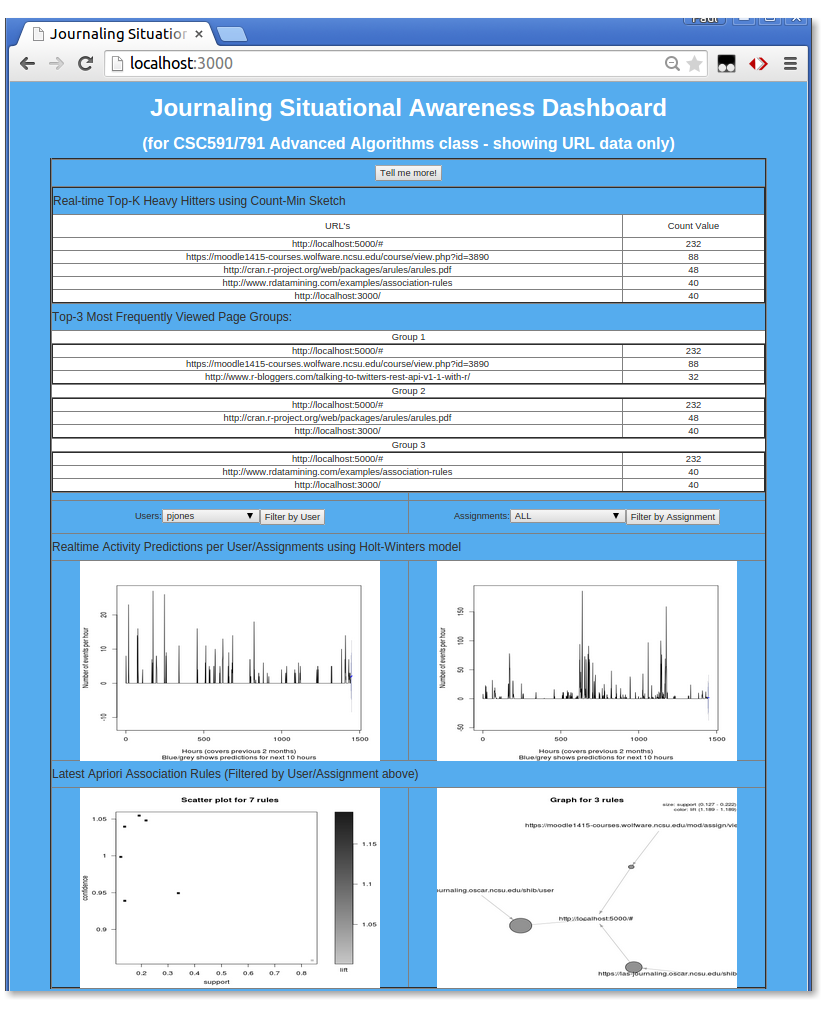
\includegraphics[width=165mm]{images/dashboard-screenshot.png}
\label{dashboard}
\caption{Screenshot from the dashboard showing a snapshot of the results described in this report}
\end{figure}

\pagebreak{}

\section{Acknowledgements}

\begin{itemize}
\item (Paul) The Holt-Winters algorithm implementation in R, described in section 2.4, was built upon my group's implementation for Project P3.
\item (Kshitij) The Algorithm described in section 2.4 for top-n frequent-item set extraction and top-k frequent URLs was built upon a similar algorithm in \cite{agrawal1994fast} (page 6).
\item (Paul) Figure 1 was derived in part from an earlier diagram created by me for LAS research.
\item (Paul) A short conversation with Claude (shsu3) on April 28th gave me some of the background information for the first paragraph of section 3.3.3.
\item (Paul) I discussed the Sequitor algorithm with Bill Szewczyk on April 30th, which helped inform my description of the algorithm in section 3.3.4.
\end{itemize}

\pagebreak

\bibliographystyle{abbrv}
\bibliography{capstone-journaling} 

\end{document}
